\chapter{Structure Beyond Linearity}
\label{ch:structure-beyond-linearity}

A failed linear baseline does not merely say the task is harder than expected. More often, it says something specific about the kind of structure that is missing. On a first pass, three possibilities matter most. Sometimes the missing structure is conditional and region-specific. Sometimes the current representation should be used differently because geometry or another simple supervised assumption matters more than one weighted sum captured. And sometimes the real task is not supervised prediction at all but exploratory organization. This chapter is about reading that failure correctly so that the next model family is chosen for a structural reason rather than out of habit.

The central task is diagnostic. The chapter opens with a small selection schema: branching structure, geometry within the current representation, or unlabeled organization. Trees, nearest neighbors, clustering, and dimensionality reduction supply that first map. Support vector machines and Naive Bayes appear as later refinements rather than as equal-weight answers from page one. By the end, the reader should be able to name what the linear model missed and justify the next family for that reason.

\begin{practicalnote}
\textbf{Core path.} In a first course, keep the required path narrow: trees and ensembles for branching logic, nearest neighbors for supervised geometry, and clustering or PCA for unlabeled organization or compression. SVMs and Naive Bayes are useful refinement previews, but they should not turn the chapter into a catalog of methods.
\end{practicalnote}

\section{Opening Question: What Kind of Structure Is Missing?}

Return to the early student-support setting. Suppose a university wants to identify students who may need extra support. One group of at-risk students may have very low attendance but acceptable quiz scores. Another may attend regularly yet miss many deadlines. A single weighted sum blurs those patterns together. A branching rule describes them more naturally: if attendance is very low, flag the student; otherwise, if late submissions are frequent, flag the student; otherwise, do not.

That rule is not merely ``nonlinear.'' It is region-specific. Different logic applies in different parts of the feature space. That is one possible answer to a failed baseline.

But it is not the only answer. Sometimes the right story is not branching at all but a different use of the current feature space: similar examples might borrow judgment from one another, or a later stricter margin-based or probabilistic baseline might be needed. And sometimes labels are absent and the job is exploratory organization rather than supervised prediction.

The opening question of the chapter should therefore be stated bluntly:

\begin{center}
\emph{When the linear baseline fails, is the missing structure mainly branching logic, supervised geometry in the current representation, or unlabeled organization?}
\end{center}

Everything that follows refines that smaller question. The chapter later splits the supervised-geometry branch into more specialized options, but the opening map should stay compact.

\section{A Small Structural Map Before the Methods}

Before naming model families, name the diagnostic.

The representation card from Bridge~I recorded what counts as an example and what its coordinates mean. The structural diagnostic asks what that representation \emph{missed}---and which model family can recover what is missing.

Before changing model families, state what structural mismatch the baseline has revealed. On a first pass, do not sort among six method names. Sort among three structural stories. If the task sounds like branching logic, think trees. If prediction should come from the geometry of nearby cases or some other supervised assumption inside the current representation, start with the geometry branch and refine later. If labels are absent and you are looking for organization or compression, think clustering or dimensionality reduction.

\begin{table}[t]
\centering
\small
\setlength{\tabcolsep}{4pt}
\begin{tabular}{L{2.9cm}L{2.9cm}L{4.15cm}}
\toprule
First-pass structural mismatch & Stable first answer & What to learn first \\
\midrule
Conditional thresholds and interactions & Trees and tree ensembles & Different rules in different regions of feature space \\
Supervised prediction, but the current representation should be used through geometry or another simple assumption & Nearest neighbors first; SVM and Naive Bayes later as refinements & Learn to ask whether the current coordinates already support a justified supervised rule \\
Unlabeled organization & Clustering and dimensionality reduction & Summarize groupings, directions of variation, or lower-dimensional views without labels \\
\bottomrule
\end{tabular}
\caption{The opening map is intentionally small. The point is to stabilize the diagnosis before splitting one branch into narrower later method choices.}
\label{tab:structure-map}
\end{table}

Keep one tiny student-profile cloud in mind throughout the chapter. Students A and B have around 50{,}000 clicks and at most one late submission and look safe; students C and D have around 20{,}000 clicks and four or five late submissions and look risky. On the first pass, read that cloud three ways: as threshold logic for trees, as geometry for supervised methods that trust the current representation, or as grouping and variation for unsupervised methods. Later sections show how SVMs and Naive Bayes sharpen the supervised branch in different ways. The better question is not ``Which stronger model should we try next?'' but ``What specific structure did the baseline miss?''

Read the chapter left to right as a diagnostic tree: first identify the missing structure, then choose the family that naturally expresses it.

\section{Method Selection by Missing Structure}

Moving beyond the linear baseline is not a random choice. It is a diagnostic response to a specific structural deficit. The first decision should stay coarse: branching logic, supervised structure in the current representation, or unlabeled organization. Only after that coarse diagnosis is stable should the reader split the supervised branch into narrower options.

\paragraph{Conditional thresholds and interactions.} If the decision rule sounds like branching logic---``if this condition holds \emph{and} that other condition holds, the outcome changes''---a linear model will fail because it cannot express regions. Trees are the natural response. They partition the input space recursively, and each leaf can express a different rule. This is the right structure for problems like loan approval, customer segmentation, or academic risk scoring, where the relevant factors interact nonlinearly across subgroups.

\paragraph{Local similarity.} If prediction should come from nearby examples---because similar students, products, or sensor readings tend to have similar outcomes---the structure is geometric rather than partitioned. Nearest-neighbor methods are the natural response. They delegate intelligence to the geometry of the feature space instead of building a global rule. This is the right structure when the decision boundary is irregular but local smoothness is plausible.

\paragraph{No labels: organization or compression.} If labels are absent and the goal is to discover natural groups, reduce dimensions for visualization, or build a compact intermediate representation, clustering or dimensionality reduction is the right response. These methods ask different questions than supervised methods, and they belong when the task is exploratory rather than predictive.

SVMs and Naive Bayes belong later in the same diagnostic story, but not at the same pedagogical level as the opening split. Once the task is clearly supervised and the current representation is worth defending, SVMs ask for a wide-margin separator and Naive Bayes asks whether simple class-conditional assumptions yield a useful probabilistic baseline. Those refinements matter, but the chapter works better when they arrive after the smaller map is stable.

\begin{table}[t]
\centering
\small
\setlength{\tabcolsep}{4pt}
\begin{tabular}{L{3.1cm}L{2.75cm}L{4.1cm}}
\toprule
Diagnostic stage & Method family & What it contributes \\
\midrule
First-pass: threshold interactions, region-specific rules & Trees and ensembles & Different rules in different parts of feature space \\
First-pass: supervised geometry should drive prediction & Nearest neighbors & Borrow labels from nearby examples under a chosen metric \\
Later refinement of the geometry branch & SVM & Robust boundary when a defended representation should support wide-margin separation \\
Later probabilistic refinement within supervised modeling & Naive Bayes & Generative baseline; interpretable, fast, and useful when simple class-conditional assumptions are plausible \\
First-pass: no labels; seek grouping or compression & Clustering, PCA & Organize or compress without a target label \\
\bottomrule
\end{tabular}
\caption{Method selection should follow structural diagnosis, but the early chapter should not force every family into the reader's first decision.}
\label{tab:method-selection}
\end{table}

The wrong version of this reasoning is method shopping: trying several families in sequence and reporting the one with the best number, with no explanation of why that family should work. The right version names the structural mismatch first and selects a method because it addresses that mismatch. The discipline makes model choice defensible and experiments interpretable. It also helps rule methods out for good reasons instead of trying everything indiscriminately.

\section{Trees: Conditional Logic and Region-Specific Rules}

\begin{figure}[t]
\centering
\definecolor{c4cls1}{RGB}{56,103,170}
\definecolor{c4cls2}{RGB}{184,92,16}
\definecolor{c4regA}{RGB}{220,233,251}
\definecolor{c4regB}{RGB}{254,237,215}
\definecolor{c4regC}{RGB}{210,238,220}
\resizebox{\linewidth}{!}{%
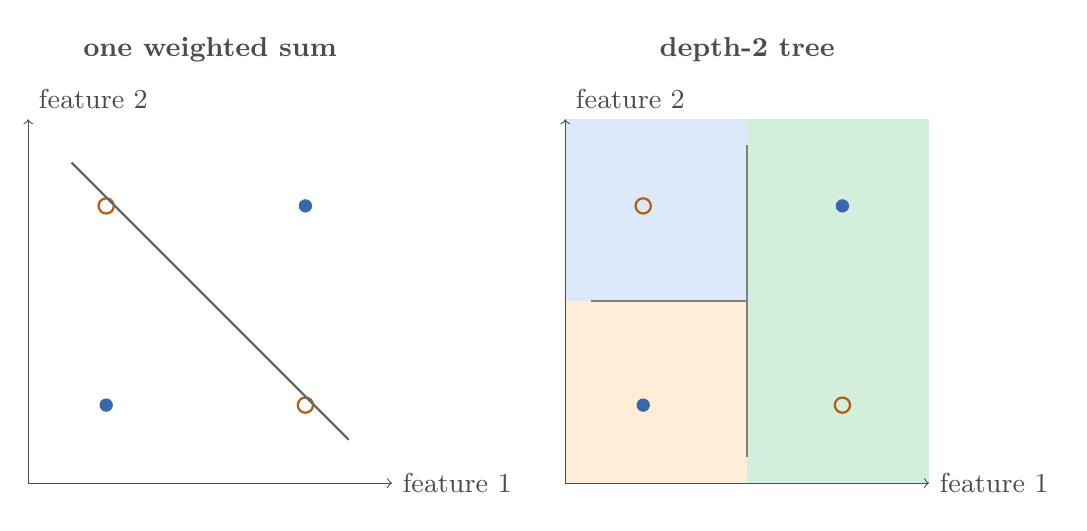
\begin{tikzpicture}[font=\small, scale=1.1, every node/.style={transform shape}]
%% Panel A: one linear separator
\begin{scope}
  \draw[->,black!70] (0,0) -- (4.2,0) node[right] {feature 1};
  \draw[->,black!70] (0,0) -- (0,4.2) node[above right] {feature 2};
  \filldraw[fill=c4cls1,draw=c4cls1] (0.9,0.9) circle (2pt);
  \filldraw[fill=c4cls1,draw=c4cls1] (3.2,3.2) circle (2pt);
  \draw[c4cls2,thick] (0.9,3.2) circle (2.5pt);
  \draw[c4cls2,thick] (3.2,0.9) circle (2.5pt);
  \draw[black!60,thick] (0.5,3.7) -- (3.7,0.5);
  \node[black!70, font=\small\bfseries] at (2.1,5.0) {one weighted sum};
\end{scope}
%% Panel B: depth-2 tree regions
\begin{scope}[xshift=6.2cm]
  \fill[c4regA] (0,2.1) rectangle (2.1,4.2);
  \fill[c4regB] (0,0)   rectangle (2.1,2.1);
  \fill[c4regC] (2.1,0) rectangle (4.2,4.2);
  \draw[->,black!70] (0,0) -- (4.2,0) node[right] {feature 1};
  \draw[->,black!70] (0,0) -- (0,4.2) node[above right] {feature 2};
  \filldraw[fill=c4cls1,draw=c4cls1] (0.9,0.9) circle (2pt);
  \filldraw[fill=c4cls1,draw=c4cls1] (3.2,3.2) circle (2pt);
  \draw[c4cls2,thick] (0.9,3.2) circle (2.5pt);
  \draw[c4cls2,thick] (3.2,0.9) circle (2.5pt);
  \draw[black!50,thick] (2.1,0.3) -- (2.1,3.9);
  \draw[black!50,thick] (0.3,2.1) -- (2.1,2.1);
  \node[black!70, font=\small\bfseries] at (2.1,5.0) {depth-2 tree};
\end{scope}
\end{tikzpicture}%
}
\caption{The same 2D dataset can defeat a single linear separator and still invite shallow, region-specific tree rules. The structural difference is global score versus local branching; additional splits can refine the partition further.}
\label{fig:linear-vs-tree}
\end{figure}

\begin{definition}[Decision Tree]
A decision tree is a model that predicts by recursively partitioning the feature space. Each internal node asks a question about the input, each branch corresponds to an answer, and each leaf produces a prediction.
\end{definition}

The right headline for trees is not ``nonlinear model.'' It is this: a tree is a model for conditional logic. Picture conditions and regions, not coefficients with a more complicated curve wrapped around them.

The simplest mental model is a flowchart. A tree starts at the root and repeatedly asks questions:
\begin{itemize}[leftmargin=*]
\item Is attendance less than 70\%?
\item Is the number of late assignments greater than 2?
\item Is the neighborhood in the set \{A, C, D\}?
\end{itemize}
Depending on the answer, the example travels down one branch or another until it reaches a leaf. The leaf contains either a class label, a class-probability estimate, or a numeric prediction.

Trees capture nonlinear behavior without forcing us to hand-engineer every interaction. A feature can matter in one branch and become irrelevant in another. That makes trees especially natural when the task involves threshold-like behavior or region-specific rules.

The same cloud that appears later in the k-NN and unsupervised sections can already be read this way: the tree is looking for a threshold on lateness, not a single line that explains everything at once.

\subsection{Choosing a Split}

A tree is built by choosing splits that make the resulting child nodes ``purer'' than the parent. For classification, one common measure of impurity is the Gini impurity:
\[
G = 1 - \sum_{k} p_k^2,
\]
where $p_k$ is the fraction of examples in the node that belong to class $k$. A pure node containing only one class has impurity zero. Mixed nodes have higher impurity.

\begin{prereqbridge}
If the impurity formula looks unfamiliar, the idea is simple: a good split creates children that are more homogeneous than the parent. The formula scores that intuition.
\end{prereqbridge}

\begin{mathlens}
For binary classification, if the fraction of positive examples in a node is $p$, then the Gini impurity becomes
\[
G = 1 - p^2 - (1-p)^2 = 2p(1-p).
\]
This is 0 when $p=0$ or $p=1$, and largest at $p=0.5$. That is why pure nodes feel ``finished'' and evenly mixed nodes feel maximally impure.
\end{mathlens}

For regression trees, the objective is analogous but numeric: each split reduces variance or squared error in the target values within each child node. The recursive structure stays the same even though the leaf predictions differ.

\begin{table}[t]
\centering
\begin{tabular}{>{\centering}p{1.5cm}>{\centering}p{2.4cm}>{\centering}p{2.4cm}>{\centering\arraybackslash}p{2.7cm}}
\toprule
Student & Attendance rate & Late submissions & At risk? \\
\midrule
1 & 0.52 & 5 & yes \\
2 & 0.58 & 4 & yes \\
3 & 0.61 & 4 & yes \\
4 & 0.68 & 3 & no \\
5 & 0.72 & 1 & no \\
6 & 0.78 & 2 & no \\
7 & 0.81 & 3 & yes \\
8 & 0.88 & 1 & no \\
\bottomrule
\end{tabular}
\caption{A tiny tree-building dataset is enough to show what ``choosing a split'' means numerically.}
\label{tab:tree-split-data}
\end{table}

In Table~\ref{tab:tree-split-data}, the parent node contains four risky students and four non-risky students, so the parent Gini impurity is
\[
G_{\text{parent}} = 1 - \left(\frac{4}{8}\right)^2 - \left(\frac{4}{8}\right)^2 = 0.5.
\]

Now compare two candidate root splits:
\begin{itemize}[leftmargin=*]
\item \texttt{attendance rate} $\le 0.65$
\item \texttt{late submissions} $\le 1.5$
\end{itemize}

For the attendance split, the left child holds three risky students and no safe ones, so its impurity is 0. The right child holds one risky student and four safe ones, so its impurity is
\[
1 - \left(\frac{1}{5}\right)^2 - \left(\frac{4}{5}\right)^2 = 0.32.
\]
The weighted child impurity is therefore
\[
\frac{3}{8}(0) + \frac{5}{8}(0.32) = 0.20,
\]
so the impurity reduction is
\[
0.50 - 0.20 = 0.30.
\]

For the late-submission split at 1.5, the left child holds two safe students and no risky ones, so its impurity is again 0. The right child holds four risky students and two safe students, so its impurity is
\[
1 - \left(\frac{4}{6}\right)^2 - \left(\frac{2}{6}\right)^2 \approx 0.44.
\]
The weighted child impurity is
\[
\frac{2}{8}(0) + \frac{6}{8}(0.44) \approx 0.33,
\]
so the impurity reduction is only about
\[
0.50 - 0.33 = 0.17.
\]

The attendance split is therefore better at the root.

\begin{codeexample}[caption={From scratch: computing Gini impurity reduction for one candidate split}]
def gini(labels):
    n = len(labels)
    if n == 0:
        return 0.0
    counts = {}
    for label in labels:
        counts[label] = counts.get(label, 0) + 1
    return 1.0 - sum((c / n) ** 2 for c in counts.values())

# Student at-risk labels from the chapter dataset
left_labels  = ["yes", "yes", "yes"]          # attendance <= 0.65
right_labels = ["no", "no", "no", "no", "yes"] # attendance > 0.65
parent_labels = left_labels + right_labels

n_total = len(parent_labels)
n_left  = len(left_labels)
n_right = len(right_labels)

parent_impurity = gini(parent_labels)
left_impurity   = gini(left_labels)
right_impurity  = gini(right_labels)
weighted_child  = (n_left / n_total) * left_impurity \
                + (n_right / n_total) * right_impurity
reduction = parent_impurity - weighted_child

print("parent impurity:", round(parent_impurity, 4))
print("left  impurity:", round(left_impurity, 4))
print("right impurity:", round(right_impurity, 4))
print("weighted reduction:", round(reduction, 4))
\end{codeexample}

\begin{figure}[t]
\centering
\definecolor{c4impA}{RGB}{220,233,251}
\definecolor{c4impB}{RGB}{56,103,170}
\definecolor{c4impLineA}{RGB}{56,103,170}
\resizebox{\linewidth}{!}{%
\begin{tikzpicture}[font=\small]
%% Parent node
\begin{scope}
  \node[black!70, font=\small\bfseries] at (0,2.9) {Parent node};
  \fill[c4impA]  (-1.8,0) rectangle (0.0,2.0);
  \fill[c4impB]  (0.0,0)  rectangle (1.8,2.0);
  \draw[black!50] (-1.8,0) rectangle (1.8,2.0);
  \draw[black!40] (0,0) -- (0,2.0);
  \node[white, font=\small\bfseries] at (0.9,1.0) {$G=0.50$};
  \node[black!70, font=\footnotesize] at (-0.9,-0.35) {risk};
  \node[black!70, font=\footnotesize] at (0.9,-0.35) {safe};
\end{scope}
%% After split
\begin{scope}[xshift=5.3cm]
  \definecolor{c4impGreen}{RGB}{26,112,64}
  \definecolor{c4impGreenBg}{RGB}{210,238,220}
  \node[black!70, font=\small\bfseries] at (0,2.9) {After better split};
  %% Left child: pure
  \fill[c4impA] (-2.2,0) rectangle (-0.8,2.0);
  \draw[black!50] (-2.2,0) rectangle (-0.8,2.0);
  \node[white, font=\small\bfseries] at (-1.5,1.0) {$G=0$};
  \node[black!70, font=\footnotesize] at (-1.5,-0.35) {left child};
  %% Right child: mixed but better
  \fill[c4impB]  (0.2,0) rectangle (2.8,2.0);
  \fill[c4impA] (0.2,0) rectangle (0.72,2.0);
  \draw[black!50] (0.2,0) rectangle (2.8,2.0);
  \draw[black!30] (0.72,0) -- (0.72,2.0);
  \node[c4impLineA, font=\small\bfseries] at (1.5,1.0) {$G=0.32$};
  \node[black!70, font=\footnotesize] at (1.5,-0.35) {right child};
\end{scope}
\end{tikzpicture}%
}
\caption{Impurity reduction is not mystical. A useful split creates children that are more class-homogeneous than the parent node.}
\label{fig:impurity-before-after}
\end{figure}

\subsection{A Tree and Its Regions}

The split calculation tells us which question to ask. The tree itself shows how the space is partitioned.

\begin{figure}[t]
\centering
\definecolor{c4decBg}{RGB}{220,233,251}
\definecolor{c4decLine}{RGB}{56,103,170}
\definecolor{c4riskBg}{RGB}{254,216,216}
\definecolor{c4riskLine}{RGB}{180,40,40}
\definecolor{c4safeBg}{RGB}{210,238,220}
\definecolor{c4safeLine}{RGB}{26,112,64}
\definecolor{c4regRisk}{RGB}{254,216,216}
\definecolor{c4regSafe}{RGB}{210,238,220}
\definecolor{c4regMid}{RGB}{235,242,253}
\resizebox{\linewidth}{!}{%
\begin{tikzpicture}[font=\small]
%% ---- Flowchart ----
\begin{scope}
  \node[draw=c4decLine, fill=c4decBg, rounded corners, align=center, text=c4decLine, font=\small\bfseries]
    (root) at (0,0) {attendance\\$\le 0.65$?};
  \node[draw=c4riskLine, fill=c4riskBg, rounded corners, align=center, font=\small]
    (leftleaf) at (-2.1,-1.8) {risk};
  \node[draw=c4decLine, fill=c4decBg, rounded corners, align=center, text=c4decLine, font=\small\bfseries]
    (rightnode) at (2.1,-1.8) {late submissions\\$> 2.5$?};
  \node[draw=c4safeLine, fill=c4safeBg, rounded corners, align=center, font=\small]
    (midleaf) at (0.8,-3.5) {safe};
  \node[draw=c4riskLine, fill=c4riskBg, rounded corners, align=center, font=\small]
    (rightleaf) at (3.4,-3.5) {risk};
  \draw[-Latex,thick,black!60] (root) -- (leftleaf);
  \draw[-Latex,thick,black!60] (root) -- (rightnode);
  \draw[-Latex,thick,black!60] (rightnode) -- (midleaf);
  \draw[-Latex,thick,black!60] (rightnode) -- (rightleaf);
  \node[font=\footnotesize,black!60] at (-1.1,-0.9) {yes};
  \node[font=\footnotesize,black!60] at (1.2,-0.9)  {no};
  \node[font=\footnotesize,black!60] at (1.6,-2.7)  {no};
  \node[font=\footnotesize,black!60] at (3.0,-2.7)  {yes};
\end{scope}
%% ---- Feature-space regions ----
\begin{scope}[xshift=6.8cm]
  \fill[c4regRisk] (0,0)   rectangle (1.7,4.0);
  \fill[c4regSafe] (1.7,0) rectangle (4.0,2.5);
  \fill[c4regMid]  (1.7,2.5) rectangle (4.0,4.0);
  \draw[->,black!70] (0,0) -- (4.5,0) node[right] {attendance};
  \draw[->,black!70] (0,0) -- (0,4.2) node[above] {late submissions};
  \draw[black!40,thick] (1.7,0) -- (1.7,4.0);
  \draw[black!40,thick] (1.7,2.5) -- (4.0,2.5);
  \node[c4riskLine,  font=\small\bfseries] at (0.85,3.5) {risk};
  \node[c4safeLine,  font=\small\bfseries] at (2.85,1.2) {safe};
  \node[c4decLine,   font=\small\bfseries] at (2.85,3.4) {risk};
\end{scope}
\end{tikzpicture}%
}
\caption{A tree can be read both as a flowchart and as a partition of feature space into rectangular regions. That dual picture is what makes the method legible.}
\label{fig:tree-flowchart-regions}
\end{figure}

\begin{example}[Why Trees Can Feel Natural]
Suppose two students each missed two assignments. A linear model treats those missed assignments similarly regardless of other context. A tree can make a different judgment if one student also has very low attendance while the other attends consistently and performs well on quizzes. The branching structure lets the model represent conditional logic directly.
\end{example}

\subsection{Depth, Overfitting, and Pruning}

The danger of trees is that they keep splitting until they fit noise or accidental patterns in the training data. A very deep tree can memorize small quirks of the dataset while appearing perfectly confident.

Several controls are common:
\begin{itemize}[leftmargin=*]
\item limiting the maximum depth of the tree
\item requiring a minimum number of examples in a node before splitting
\item pruning branches that do not improve validation performance
\end{itemize}

This is where Chapter~\ref{ch:evaluation-discipline} returns. A tree that keeps improving training accuracy is not necessarily improving the model we want. Validation performance decides whether additional branching is helping or merely memorizing.

\begin{figure}[t]
\centering
\definecolor{c4trainBlue}{RGB}{56,103,170}
\definecolor{c4valAmber}{RGB}{184,92,16}
\resizebox{\linewidth}{!}{%
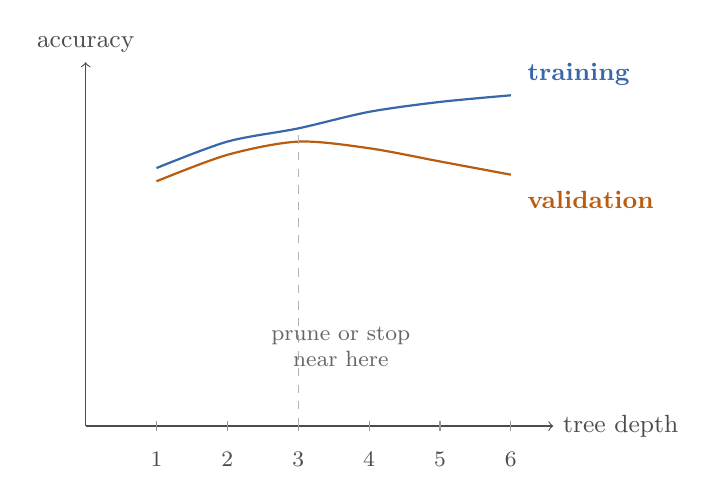
\begin{tikzpicture}[x=0.9cm,y=4.2cm,font=\small]
  \draw[->,black!70] (0,0) -- (6.6,0) node[right] {tree depth};
  \draw[->,black!70] (0,0) -- (0,1.1) node[above] {accuracy};
  \foreach \x/\lbl in {1/1,2/2,3/3,4/4,5/5,6/6}
    \draw[black!40] (\x,0.015) -- (\x,-0.015) node[below=4pt,font=\footnotesize,black!70] {\lbl};
  \draw[c4trainBlue,thick]
    plot[smooth] coordinates {(1,0.78)(2,0.86)(3,0.90)(4,0.95)(5,0.98)(6,1.00)};
  \draw[c4valAmber,thick]
    plot[smooth] coordinates {(1,0.74)(2,0.82)(3,0.86)(4,0.84)(5,0.80)(6,0.76)};
  \draw[black!30,dashed] (3,0) -- (3,0.9);
  \node[c4trainBlue, font=\small\bfseries, anchor=south west] at (6.1,1.0) {training};
  \node[c4valAmber,  font=\small\bfseries, anchor=north west] at (6.1,0.74) {validation};
  \node[align=center, font=\footnotesize, black!60] at (3.6,0.24) {prune or stop\\near here};
\end{tikzpicture}%
}
\caption{Single trees make overfitting visible quickly. Depth increases flexibility, but after a point the training gain is mostly memorization.}
\label{fig:tree-depth-curves}
\end{figure}

\begin{example}[Validation-Based Post-Pruning]
Validation-based post-pruning is a practical way to control depth:
\begin{enumerate}
\item Grow the tree to full depth on the training set, letting it fit as closely as possible.
\item Starting from the leaves and working upward, for each internal node consider replacing the subtree rooted there with a single leaf that predicts the majority class (for classification) or the mean value (for regression).
\item If validation error does not increase after the replacement, keep the pruned version; otherwise restore the subtree.
\item Repeat until no further pruning improves validation performance.
\end{enumerate}

The key insight is that the validation set, not the training set, decides which branches are worth keeping. A branch that improved training accuracy may have been fitting noise. If validation accuracy stays the same or improves when the branch is removed, the branch did not carry useful information.
\end{example}

\begin{failurebox}
A single decision tree is often unstable. Small changes in the data can produce different root splits, different branches, and therefore different stories about what matters. That is one reason tree interpretation should be treated as useful but not absolute.
\end{failurebox}

\section{From Single Trees to Ensembles: Same Structure, More Stability}

Single trees are easy to understand, but they are often noisy, high-variance models. Once the tree story is clear, the next question is not new structure but stability. Ensemble methods do not replace tree logic; they stabilize or strengthen it.

\begin{table}[t]
\centering
\small
\setlength{\tabcolsep}{3pt}
\begin{tabular}{@{}>{\raggedright\arraybackslash}p{1.67cm}>{\raggedright\arraybackslash}p{2.16cm}>{\raggedright\arraybackslash}p{2.3cm}>{\raggedright\arraybackslash}p{4.04cm}@{}}
\toprule
Model family & Main idea & Typical strength & Typical weakness \\
\midrule
Single tree & One recursive partition of the feature space & Interpretable rules and threshold logic & Unstable and easy to overfit \\
Random forest & Many diverse trees trained in parallel and averaged & Strong tabular performance with lower variance & Less interpretable than a single tree \\
Boosted trees & Trees trained sequentially to correct earlier errors & Often very strong accuracy on structured data & More tuning-sensitive and easier to overfit if pushed too far \\
\bottomrule
\end{tabular}
\caption{Students often blur all tree-based methods together. The point of this comparison is to keep the workflows distinct.}
\label{tab:tree-ensemble-comparison}
\end{table}

\subsection{Why Averaging Mainly Reduces Variance}

A single decision tree is a low-bias model: with enough depth it can represent almost any boundary in its training data. But it is also high-variance. A small change in the training sample---a few swapped examples---can produce a different root split, different branches, and a different story about what matters. The tree reacts strongly to the accidents of the data it saw.

Averaging many independent trees does not change each tree's bias---each is still fitting the same underlying problem---but it does reduce variance. Predictions that fluctuate differently across trees cancel in the average, leaving the stable signal most trees agree on.

Think of it this way. One panelist's opinion about whether a student is at risk is noisy and idiosyncratic. The average of fifty panelists who independently reviewed the same evidence is far more reliable. Their individual errors are uncorrelated enough to wash out, and the shared signal survives.

\begin{figure}[t]
\centering
\definecolor{c4ensCls1}{RGB}{56,103,170}
\definecolor{c4ensCls2}{RGB}{184,92,16}
\definecolor{c4ensBnd}{RGB}{80,80,80}
\resizebox{\linewidth}{!}{%
\begin{tikzpicture}[font=\small,
  box/.style={draw, rounded corners, fill=black!4, minimum width=2.0cm, minimum height=0.7cm, align=center}
]
%% Left: individual noisy boundaries
\begin{scope}
  \node[font=\small\bfseries, black!70] at (2.0,4.6) {individual trees};
  \draw[->,black!70] (0,0) -- (4.2,0) node[right] {$x_1$};
  \draw[->,black!70] (0,0) -- (0,4.2) node[above] {$x_2$};
  \filldraw[fill=c4ensCls1,draw=c4ensCls1] (0.7,0.8) circle (2pt);
  \filldraw[fill=c4ensCls1,draw=c4ensCls1] (1.1,1.5) circle (2pt);
  \filldraw[fill=c4ensCls1,draw=c4ensCls1] (0.9,2.8) circle (2pt);
  \draw[c4ensCls2,thick] (2.8,1.0) circle (2.5pt);
  \draw[c4ensCls2,thick] (3.3,2.1) circle (2.5pt);
  \draw[c4ensCls2,thick] (3.0,3.3) circle (2.5pt);
  \draw[black!40,thick]         (1.8,0.2) -- (1.4,4.0);
  \draw[black!40,thick,dashed]  (2.3,0.3) -- (2.6,4.0);
  \draw[black!40,thick,dotted]  (1.2,0.2) -- (1.9,4.0);
  \node[align=center, font=\footnotesize, black!60] at (2.0,-0.55) {three different\\boundaries};
\end{scope}
%% Arrow
\draw[-Latex,thick,black!50] (4.5,2.1) -- (5.5,2.1);
%% Right: averaged boundary
\begin{scope}[xshift=6.0cm]
  \node[font=\small\bfseries, black!70] at (2.0,4.6) {averaged boundary};
  \draw[->,black!70] (0,0) -- (4.2,0) node[right] {$x_1$};
  \draw[->,black!70] (0,0) -- (0,4.2) node[above] {$x_2$};
  \filldraw[fill=c4ensCls1,draw=c4ensCls1] (0.7,0.8) circle (2pt);
  \filldraw[fill=c4ensCls1,draw=c4ensCls1] (1.1,1.5) circle (2pt);
  \filldraw[fill=c4ensCls1,draw=c4ensCls1] (0.9,2.8) circle (2pt);
  \draw[c4ensCls2,thick] (2.8,1.0) circle (2.5pt);
  \draw[c4ensCls2,thick] (3.3,2.1) circle (2.5pt);
  \draw[c4ensCls2,thick] (3.0,3.3) circle (2.5pt);
  \draw[c4ensBnd,very thick] (1.9,0.2) -- (2.0,4.0);
  \node[align=center, font=\footnotesize, black!60] at (2.0,-0.55) {stable consensus\\boundary};
\end{scope}
\end{tikzpicture}%
}
\caption{Individual trees produce noisy, jittery boundaries that vary with the training sample. Averaging many diverse trees smooths those fluctuations while preserving the underlying signal.}
\label{fig:ensemble-variance-reduction}
\end{figure}

\begin{mathlens}
Suppose $T$ trees each produce an independent prediction with variance $\sigma^2$. The variance of their average is
\[
\operatorname{Var}\!\left(\frac{1}{T}\sum_{t=1}^{T} \hat{y}_t\right) = \frac{\sigma^2}{T}.
\]
Averaging $T$ uncorrelated estimators reduces variance by a factor of $T$ while leaving the expected prediction unchanged. Trees are not perfectly uncorrelated in practice, so the gain is smaller than $1/T$, but the direction is the same: more diverse trees, lower variance.
\end{mathlens}

\paragraph{Diversity is what makes averaging work.} The variance-reduction argument rests on one critical assumption: the trees must not all make the same mistakes. If every tree in the ensemble produces the same error on the same examples, averaging changes nothing. The average of ten identical wrong answers is still a wrong answer.

This is why random forests introduce two sources of randomness deliberately. First, each tree is trained on a bootstrap resample---a training sample drawn with replacement so some examples repeat and others are left out---so trees see overlapping but different subsets of examples. Second, each split considers only a random subset of features, so trees cannot all latch onto the same dominant feature and must find different evidence.

Boosted trees achieve diversity differently and more carefully: each new tree is trained to correct the specific errors of the trees already in the ensemble. Early trees handle the easy cases; later trees focus on the residual. The sequential structure means boosted trees do not rely on random diversity; they build complementarity by design.

\begin{example}[When Averaging Fails]
Suppose a training set has a systematic labeling error: every example from a particular sensor type is mislabeled. Every tree in the ensemble trains on that same biased data, and the average of their predictions inherits the same bias. Ensembles reduce variance from random sample fluctuations; they do not reduce bias from structural problems in the data itself. That is one reason error analysis on the full ensemble is still essential even when the ensemble is strong on average.
\end{example}

If you want a robust default on tabular data with minimal tuning, prefer a random forest: it is harder to badly overfit and easier to parallelize. Prefer boosted trees when you need the strongest possible accuracy on structured data and are willing to tune carefully---boosting can squeeze out more performance but is more sensitive to the number of rounds, tree depth, and learning rate. On small or noisy datasets, the safer prior is the random forest, because aggressive boosting can amplify noise when pushed too far.

\begin{figure}[t]
\centering
\definecolor{c4bagBg}{RGB}{220,233,251}
\definecolor{c4bagLine}{RGB}{56,103,170}
\definecolor{c4boostBg}{RGB}{254,237,215}
\definecolor{c4boostLine}{RGB}{184,92,16}
\definecolor{c4avgBg}{RGB}{210,238,220}
\definecolor{c4avgLine}{RGB}{26,112,64}
\resizebox{\linewidth}{!}{%
\begin{tikzpicture}[x=1cm, y=1cm,
  bagbox/.style={draw=c4bagLine,  fill=c4bagBg,  rounded corners, align=center,
                 minimum height=0.85cm, minimum width=2.0cm,
                 font=\small\bfseries, text=c4bagLine},
  bobox/.style= {draw=c4boostLine,fill=c4boostBg,rounded corners, align=center,
                 minimum height=0.85cm, minimum width=3.2cm,
                 font=\small, text=c4boostLine},
  avgbox/.style={draw=c4avgLine,  fill=c4avgBg,  rounded corners, align=center,
                 minimum height=0.85cm, minimum width=2.4cm,
                 font=\small\bfseries, text=c4avgLine},
  arrow/.style={-Latex,thick,black!60}
]
%% ---- Bagging panel ----
\begin{scope}
  \node[black!70, font=\small\bfseries] at (3.0, 2.2) {Bagging / random forest};
  %% Three parallel samples - spacing 2.5cm so boxes (2.0cm wide) never touch
  \node[bagbox] (sample1) at (0.5, 0.8) {sample 1};
  \node[bagbox] (sample2) at (3.0, 0.8) {sample 2};
  \node[bagbox] (sample3) at (5.5, 0.8) {sample 3};
  \node[bagbox] (tree1)   at (0.5,-0.8) {tree 1};
  \node[bagbox] (tree2)   at (3.0,-0.8) {tree 2};
  \node[bagbox] (tree3)   at (5.5,-0.8) {tree 3};
  \node[avgbox] (avg)     at (3.0,-2.4) {average / vote};
  \draw[arrow] (sample1) -- (tree1);
  \draw[arrow] (sample2) -- (tree2);
  \draw[arrow] (sample3) -- (tree3);
  \draw[arrow] (tree1)   -- (avg);
  \draw[arrow] (tree2)   -- (avg);
  \draw[arrow] (tree3)   -- (avg);
\end{scope}
%% ---- Boosting panel ----
\begin{scope}[xshift=9.0cm]
  \node[black!70, font=\small\bfseries] at (1.6, 2.2) {Boosting};
  \node[bobox] (t1)  at (1.6, 0.8)  {tree 1};
  \node[bobox] (t2)  at (1.6,-0.5)  {tree 2: fix residuals};
  \node[bobox] (t3)  at (1.6,-1.8)  {tree 3: fix more};
  \node[avgbox] (sum) at (1.6,-3.1) {weighted sum};
  \draw[arrow] (t1) -- (t2);
  \draw[arrow] (t2) -- (t3);
  \draw[arrow] (t3) -- (sum);
\end{scope}
\end{tikzpicture}%
}
\caption{Random forests and boosting both use trees, but they organize them differently. One reduces variance through diverse parallel trees; the other adds trees sequentially to correct mistakes.}
\label{fig:bagging-vs-boosting}
\end{figure}

\subsection{Random Forests}

A random forest trains many trees on different resampled subsets of the data and typically considers a randomized subset of features at each split. Each tree sees a slightly different view of the problem; their predictions are averaged or voted together.

The main idea is variance reduction. A single tree may overreact to quirks of the sample, while many diverse trees averaged together are more stable. Random forests often perform very well on tabular data for this reason.

\begin{advancednote}
Random forests also offer an appealing internal-validation intuition through out-of-bag examples. Because each tree is trained on a bootstrap-style resample, some training examples are left out of that tree's fit. Those left-out examples support a rough internal check without a separate validation pass. It is not a replacement for careful evaluation, but it is a useful diagnostic idea.
\end{advancednote}

\begin{codeexample}[caption={From scratch: the prediction step of a random forest}]
def majority_vote(votes):
    counts = {}
    for v in votes:
        counts[v] = counts.get(v, 0) + 1
    return max(counts, key=counts.get)

def forest_predict(trees, example):
    # Each tree is an object with a .predict() method
    votes = [tree.predict(example) for tree in trees]
    return majority_vote(votes)

# Suppose we have a list of already-trained tree objects
# and one new student profile to classify
new_student = {"attendance": 0.55, "late_submissions": 4}

prediction = forest_predict(trained_trees, new_student)
print("ensemble prediction:", prediction)

# The ensemble vote might look like:
#   tree 1 -> "yes"
#   tree 2 -> "yes"
#   tree 3 -> "no"
#   tree 4 -> "yes"
#   tree 5 -> "yes"
# majority_vote returns "yes"
\end{codeexample}

\subsection{Boosted Trees}

Boosting takes a different approach. Instead of averaging many independent trees, it trains a sequence of trees in which each new tree focuses on the mistakes of the current ensemble. The result is often a highly accurate model that builds complexity gradually.

Boosting is powerful, but it requires careful tuning. If the trees are too strong or the sequence is pushed too far, the ensemble overfits. The educational point is that ensembles improve trees not by abandoning recursive partitioning but by controlling how many trees are combined and how they share the work.

\begin{example}[Structured Ensembles in Weather Forecasting]
NOAA-supported work on storm-scale severe-weather guidance has compared tree ensembles with logistic baselines in the Warn-on-Forecast setting \citep{flora2021}. It is a good structured-ensemble example because the data is structured, the interactions are real, and the ensemble story is not hype-driven. The model family is chosen because the problem structure rewards it.
\end{example}

Tree ensembles keep the branching story and reduce its instability. The next family addresses a different situation: the representation already makes the classes look roughly separable, and the main question is how to place a robust boundary rather than how to build region-specific rules.

\section{Margin-Based Classification: Support Vector Machines}

Trees handle region-specific logic. Nearest neighbors handle local similarity. Margin-based classification handles a different geometric story: the classes already look roughly linearly separable in the current representation, and the best separator is the one that stays as far as possible from the nearest training points. SVMs are therefore the geometric continuation of the global-separator idea from the linear baseline, with a stricter robustness preference.

\begin{definition}[Support Vector Machine]
A support vector machine is a classifier that chooses a separating hyperplane with the largest margin between classes. In the hard-margin picture, the \emph{support vectors} are the training points that lie on the margin. In the soft-margin picture, they are the examples whose margin constraints are active, including points on the margin and points that violate it. Those are the examples that actually determine the fitted boundary. When perfect separation is not realistic, the \emph{soft-margin} version allows some violations and penalizes them instead of demanding zero mistakes.
\end{definition}

The geometric idea is simple. Many separating lines may correctly classify the same data; an SVM prefers the line most robust to small perturbations. The examples with active margin constraints are the \emph{support vectors}---the points that actually define the margin.

\begin{mathlens}
For binary labels \(y_i \in \{-1,+1\}\) and a linear score \(f(x)=w^\top x+b\), the hard-margin SVM solves
\[
\begin{aligned}
\min_{w,b} \quad &\frac{1}{2}\|w\|_2^2 \\
\text{subject to} \quad &y_i f(x_i) \ge 1 \text{ for all } i.
\end{aligned}
\]
The soft-margin form adds slack variables \(\xi_i\) and a penalty:
\[
\begin{aligned}
\min_{w,b,\xi} \quad &\frac{1}{2}\|w\|_2^2 + C\sum_i \xi_i \\
\text{subject to} \quad &y_i f(x_i) \ge 1-\xi_i,\ \xi_i \ge 0.
\end{aligned}
\]
This is equivalent to minimizing the unconstrained hinge-loss objective:
\[
\frac{1}{2}\|w\|_2^2 + C\sum_i \max(0, 1-y_i f(x_i)).
\]
The first term prefers a wide margin. The second term is the \emph{hinge loss}, weighted by \(C\): it is zero when an example is safely beyond the margin and grows linearly when that example falls inside the margin or on the wrong side of the boundary.
\end{mathlens}

\begin{theorem}[Maximum margin is minimum norm under canonical scaling]
If a separating hyperplane is written in canonical scaling so that
\[
\min_i y_i(w^\top x_i+b)=1,
\]
then its geometric margin is $1/\|w\|_2$. Therefore maximizing the geometric margin is equivalent to minimizing $\|w\|_2^2$ under the canonical SVM constraints \citep{cortes1995}.
\end{theorem}

\begin{proof}
The geometric margin of the separator is
\[
\min_i \frac{y_i(w^\top x_i+b)}{\|w\|_2}.
\]
Under canonical scaling, the numerator's minimum is exactly $1$, so the margin becomes $1/\|w\|_2$. A separator with larger geometric margin therefore has smaller norm, and minimizing the norm under the same constraints maximizes the margin.
\end{proof}

\begin{example}[A One-Dimensional Margin Choice]
Suppose the negative class lies at \(x=0\) and \(x=1\), and the positive class lies at \(x=3\) and \(x=4\). Any threshold between 1 and 3 separates the classes. A threshold at \(x=1.5\) is valid, but its nearest points are only 0.5 away. A threshold at \(x=2\) is also valid, and its nearest points are 1 unit away. The second separator has the larger margin, so it is the better SVM-style choice.
\end{example}

\begin{codeexample}[caption={A subgradient-style hinge-loss sketch for a linear SVM}]
initialize w and b
for each pass over the data:
    for each example (x_i, y_i):
        margin = y_i * (dot(w, x_i) + b)
        if margin < 1:
            # inside the margin or on the wrong side
            w = (1 - eta) * w + eta * C * y_i * x_i
            b = b + eta * C * y_i
        else:
            # only the margin term applies
            w = (1 - eta) * w

# The sketch shows the core tradeoff:
# widen the margin, but pay for violations.
\end{codeexample}

This is a subgradient-style sketch for intuition, not a production SVM solver. Its job is to make the update direction legible, not to reproduce the exact optimization routines used in mature libraries.

An SVM fits when the current representation already makes the classes look close to linearly separable and you want a robust, wide-margin boundary that will not flip under small perturbations. A tree or tree ensemble is the better choice when the task is really region-specific threshold logic or when different subgroups obey different rules. If the geometry itself is poor, learned representations come first: an SVM cannot invent missing features or repair a bad embedding.

\begin{failurebox}
An SVM is not a replacement for representation learning. If the problem needs many local rules, structured interactions, or a better geometry before any separator makes sense, a tree-based model or a learned representation is the more honest next step.
\end{failurebox}

\section{Naive Bayes: Probability as Structure (Preview)}
\label{sec:naive-bayes-ch4}

Trees exploit region-specific logic. Ensembles reduce variance by averaging. SVMs find wide-margin boundaries. Naive Bayes adds one more structural diagnosis: sometimes the useful baseline is not a more flexible boundary but a simple model of what examples from each class tend to look like.

This chapter needs only the design move. A discriminative classifier asks, ``given this input, which class should it receive?'' A generative classifier asks, ``for each class, how surprising would this input be?'' Naive Bayes is the simplest version of the second idea: estimate class frequencies, estimate simple feature patterns within each class, and choose the class that makes the observed features most plausible. The full probabilistic treatment---formal model, calibration, and the connection to latent-variable methods---appears in Chapter~\ref{ch:probabilistic-models}.

The name is a warning label. Naive Bayes assumes that features are conditionally independent given the class. That is usually false: student messages mentioning ``deadline'' are more likely also to mention ``extension,'' and dark pedestrian images are more likely to contain headlights. The assumption is still useful because it makes the baseline cheap, transparent, and surprisingly competitive when the main signal is class-conditional feature frequency rather than complex feature interaction.

\begin{warningbox}
Treat Naive Bayes as a structural baseline, not an automatically trustworthy confidence machine. Its probability outputs are often poorly calibrated because the independence assumption double-counts correlated evidence. Low likelihood under all classes can suggest unfamiliar input, but it is a hypothesis to validate, not proof that the example is truly out of distribution.
\end{warningbox}

\begin{example}[Naive Bayes for Student Support Triage]
The course-support team builds a Naive Bayes classifier as a first probabilistic baseline for triaging student messages into ROUTINE, CONCERNING, and URGENT. With a bag-of-words representation, the model learns class-specific word patterns: ``quiz'' for ROUTINE, ``deadline'' for CONCERNING, ``emergency'' for URGENT. The lesson is diagnostic. If the cheap baseline is competitive, class-conditional word patterns already carry strong signal. If it fails badly, the team should look for interactions, context, or representation structure that bag-of-words cannot express.
\end{example}

\begin{decisionbox}
\textbf{Adding Naive Bayes to the structural diagnosis.}
\begin{itemize}[leftmargin=*]
\item Try it when the task has many sparse features, limited labeled data, or a need for a transparent probabilistic baseline.
\item Compare it with logistic regression and a small tree. Each baseline fails for a different reason, and the failure pattern tells you what structure is missing.
\item Escalate to Chapter~\ref{ch:probabilistic-models} when you need calibrated probabilities, likelihood-based unfamiliar-input checks, or a broader generative-model vocabulary.
\end{itemize}
\end{decisionbox}

\section{Local Similarity: When Geometry Is the Model}

\begin{definition}[Nearest-Neighbor Method]
A nearest-neighbor method predicts for a new example by comparing it to nearby examples in the training set and borrowing information from those neighbors.
\end{definition}

This is a very different philosophy from linear models or trees. A nearest-neighbor model does not summarize the dataset in coefficients or branching rules. It stores the examples and relies on the geometry of the feature space.

That is why one sentence in this section matters more than any formula:

\begin{center}
\emph{Distance is the real model.}
\end{center}

Defending a nearest-neighbor result therefore means defending the representation and similarity rule together.

For $k$-nearest neighbors, a new point is compared to the training examples, the $k$ closest are identified, and the prediction comes from those neighbors. In classification, this is usually a majority vote; in regression, an average of target values.

\subsection{Distance Defines the Model}

The crucial choice is not only the number $k$ but the meaning of distance. Euclidean distance between two vectors $x$ and $x'$ is
\[
\|x - x'\|_2 = \sqrt{\sum_{j=1}^{d}(x_j - x'_j)^2}.
\]
This formula is easy to write and dangerous to use blindly. A feature on a much larger scale than the others can dominate the distance. Irrelevant features can drown out useful ones. If the representation does not place similar examples near one another, the nearest-neighbor method has little chance to succeed.

\begin{prereqbridge}
For nearest-neighbor methods, the distance function is part of the model, not an afterthought. ``What counts as near?'' is as important as ``what are the labels?''
\end{prereqbridge}

\begin{practicalnote}
Before applying any distance-based method to multi-feature data, plot at least the first two or three features in a scatter plot, colored by class label. Even a low-dimensional slice can reveal whether classes overlap, cluster separately, or sit on a continuum---and whether any separation is linear or requires local similarity to capture.
\end{practicalnote}

\subsection{Worked Example: Local Similarity in Student Profiles}

Suppose we classify a new student profile using past examples described by two features: total course-platform clicks and late submissions. The query student has profile $(51{,}000, 5)$---many clicks but also many late submissions. This is the shared student-profile cloud introduced earlier. Consider the following training examples:

\begin{table}[t]
\centering
\begin{tabular}{>{\centering}p{1.8cm}>{\centering}p{1.7cm}>{\centering}p{2.3cm}>{\centering\arraybackslash}p{2.7cm}}
\toprule
Profile & Clicks & Late submissions & Outcome \\
\midrule
A & 50{,}000 & 0 & safe \\
B & 52{,}000 & 1 & safe \\
C & 20{,}000 & 4 & risk \\
D & 22{,}000 & 5 & risk \\
\bottomrule
\end{tabular}
\caption{A tiny $k$-NN dataset is enough to show why scale changes the model itself.}
\label{tab:knn-scaling-data}
\end{table}

Under raw Euclidean distance, the nearest examples are A and B because the click count dominates the geometry, so the query looks safe. But if clicks are rescaled into units of tens of thousands before measuring distance, the late-submission difference matters much more, and the nearest neighbors become the risky students C and D. The predicted label flips even though the labels and raw data did not change.

\begin{mathlens}
Using the query \((51{,}000,5)\), the raw distances are approximately
\begin{align*}
d(A) &\approx 1000.0, & d(B) &\approx 1000.0, \\
d(C) &\approx 31000.0, & d(D) &\approx 29000.0.
\end{align*}
After rescaling clicks by \(10{,}000\), the same query becomes \((5.1,5)\), while the points become \(A=(5,0)\), \(B=(5.2,1)\), \(C=(2,4)\), \(D=(2.2,5)\). The scaled distances are approximately
\begin{align*}
d(A) &\approx 5.00, & d(B) &\approx 4.00, \\
d(C) &\approx 3.26, & d(D) &\approx 2.90.
\end{align*}
The nearest-neighbor order changes because the geometry changed. In $k$-NN, scaling is part of the model, not a cosmetic preprocessing choice.
\end{mathlens}

\begin{table}[t]
\centering
\small
\setlength{\tabcolsep}{4pt}
\begin{tabular}{>{\raggedright}p{3.2cm}>{\centering}p{2.5cm}>{\centering}p{1.6cm}>{\centering\arraybackslash}p{1.6cm}}
\toprule
Representation & Nearest neighbors & $k{=}1$ pred. & $k{=}3$ pred. \\
\midrule
Raw $(\text{clicks},\,\text{late})$ & B, A, D & safe & safe \\
Scaled $(\text{clicks}/10\text{,}000,\,\text{late})$ & D, C, B & risk & risk \\
\bottomrule
\end{tabular}
\caption{When a distance-based model changes after scaling, that is not an implementation detail. It is the geometry of the model changing.}
\label{tab:knn-scaling-summary}
\end{table}

\begin{codeexample}[caption={Algorithm sketch: 1-nearest neighbor on the scaled representation}]
Input: query q, labeled dataset D
best_distance = infinity
best_label = none
for each (x, y) in D:
    d = EuclideanDistance(q, x)
    if d < best_distance:
        best_distance = d
        best_label = y
return best_label, best_distance
\end{codeexample}

For comparison, the raw representation keeps clicks in their original units:
\begin{codeexample}[caption={The same 1-NN sketch on the raw representation}]
Input: raw query q_raw, raw labeled dataset D_raw
run the same nearest-neighbor loop without rescaling features
compare the returned label and distance with the scaled version
\end{codeexample}

The snippet is small on purpose. It exposes the whole method: store the examples, measure distance to each one, and borrow the label of the nearest case. Later libraries may optimize this idea, but they should not hide it.

\begin{figure}[t]
\centering
\definecolor{c4knnCls1}{RGB}{56,103,170}
\definecolor{c4knnCls2}{RGB}{184,92,16}
\definecolor{c4knnQuery}{RGB}{26,112,64}
\resizebox{\linewidth}{!}{%
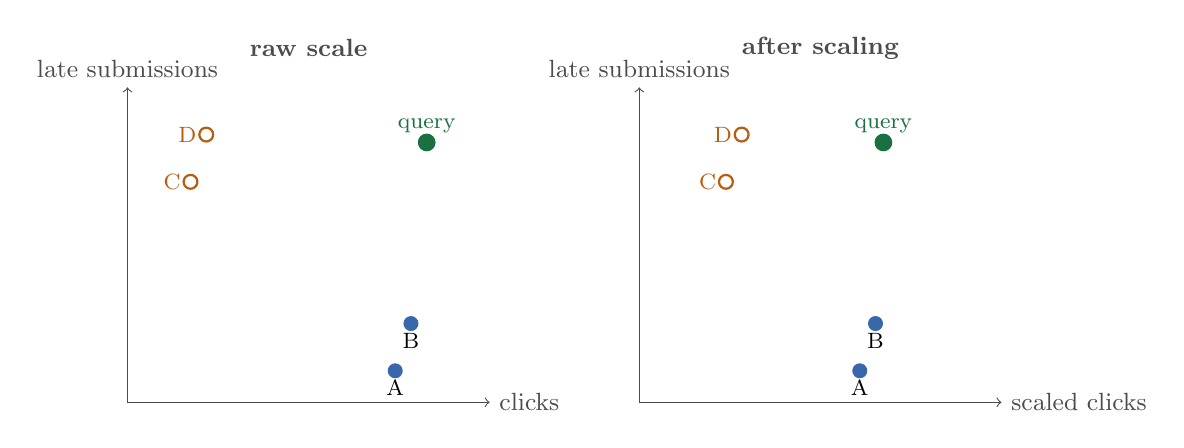
\begin{tikzpicture}[font=\small]
%% Panel A: raw scale
\begin{scope}
  \draw[->,black!70] (0,0) -- (4.6,0) node[right] {clicks};
  \draw[->,black!70] (0,0) -- (0,4.0) node[above] {late submissions};
  \filldraw[fill=c4knnCls1,draw=c4knnCls1] (3.4,0.4) circle (2.5pt) node[below,font=\footnotesize] {A};
  \filldraw[fill=c4knnCls1,draw=c4knnCls1] (3.6,1.0) circle (2.5pt) node[below,font=\footnotesize] {B};
  \draw[c4knnCls2,thick] (0.8,2.8) circle (2.5pt);
  \node[left,font=\footnotesize,c4knnCls2] at (0.8,2.8) {C};
  \draw[c4knnCls2,thick] (1.0,3.4) circle (2.5pt);
  \node[left,font=\footnotesize,c4knnCls2] at (1.0,3.4) {D};
  \filldraw[fill=c4knnQuery,draw=c4knnQuery] (3.8,3.3) circle (3pt);
  \node[above,font=\footnotesize,c4knnQuery] at (3.8,3.3) {query};
  \node[black!70,font=\small\bfseries] at (2.3,4.5) {raw scale};
\end{scope}
%% Panel B: after scaling
\begin{scope}[xshift=6.5cm]
  \draw[->,black!70] (0,0) -- (4.6,0) node[right] {scaled clicks};
  \draw[->,black!70] (0,0) -- (0,4.0) node[above] {late submissions};
  \filldraw[fill=c4knnCls1,draw=c4knnCls1] (2.8,0.4) circle (2.5pt) node[below,font=\footnotesize] {A};
  \filldraw[fill=c4knnCls1,draw=c4knnCls1] (3.0,1.0) circle (2.5pt) node[below,font=\footnotesize] {B};
  \draw[c4knnCls2,thick] (1.1,2.8) circle (2.5pt);
  \node[left,font=\footnotesize,c4knnCls2] at (1.1,2.8) {C};
  \draw[c4knnCls2,thick] (1.3,3.4) circle (2.5pt);
  \node[left,font=\footnotesize,c4knnCls2] at (1.3,3.4) {D};
  \filldraw[fill=c4knnQuery,draw=c4knnQuery] (3.1,3.3) circle (3pt);
  \node[above,font=\footnotesize,c4knnQuery] at (3.1,3.3) {query};
  \node[black!70,font=\small\bfseries] at (2.3,4.5) {after scaling};
\end{scope}
\end{tikzpicture}%
}
\caption{The same points can produce different nearest neighbors after sensible scaling. For $k$-NN, geometry is not a visualization choice. It is the model itself.}
\label{fig:knn-before-after-scaling}
\end{figure}

\begin{failurepattern}
A nearest-neighbor result can flip after a harmless-looking unit conversion or after adding one large-scale irrelevant feature. That is not random behavior. The geometry changed, so the model changed. If the notion of similarity is not defended, the prediction is not defended either.
\end{failurepattern}

Euclidean distance is not sacred either. Manhattan distance, cosine similarity, learned metrics, and domain-specific similarity functions each define a different notion of neighborhood. Changing the similarity rule changes the model.

\section{Scale, Similarity, and the Curse of Dimensionality}

The previous section gave the positive story: geometry can be the right inductive bias. This section gives the warning: geometry is fragile when the representation is poor.

As the number of features grows, distances become less informative. Many points start to look similarly far away, and local neighborhoods become hard to define meaningfully. This is one form of the curse of dimensionality.

\begin{figure}[t]
\centering
\definecolor{c4distBlue}{RGB}{56,103,170}
\definecolor{c4distAmber}{RGB}{184,92,16}
\resizebox{\linewidth}{!}{%
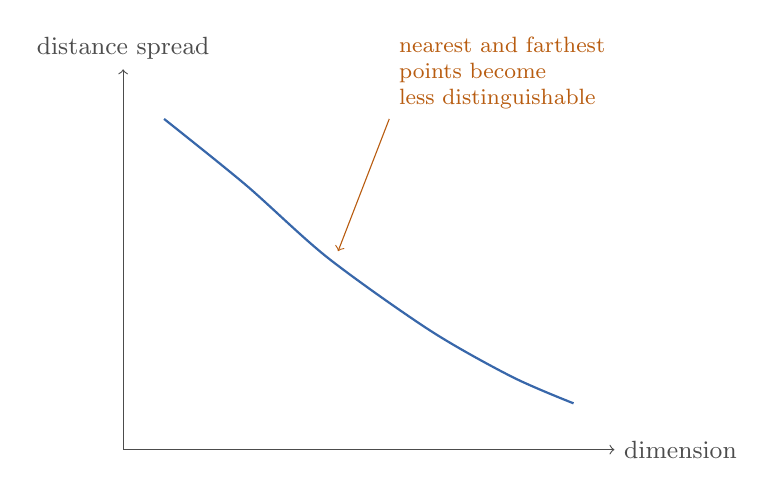
\begin{tikzpicture}[x=1.3cm, y=4.2cm, font=\small]
  \draw[->,black!70] (0,0) -- (4.8,0) node[right] {dimension};
  \draw[->,black!70] (0,0) -- (0,1.15) node[above] {distance spread};
  %% Descending curve: high spread at low dim, low spread at high dim
  \draw[c4distBlue,thick]
    plot[smooth] coordinates {(0.4,1.0)(1.2,0.80)(2.0,0.58)(3.0,0.36)(3.8,0.22)(4.4,0.14)};
  %% Annotation placed top-right, well above the curve
  \node[align=left, font=\footnotesize, c4distAmber, anchor=south west] at (2.6,1.0)
    {nearest and farthest\\points become\\less distinguishable};
  %% Arrow from annotation down to curve
  \draw[->,thin,c4distAmber] (2.6,1.0) -- (2.1,0.60);
\end{tikzpicture}%
}
\caption{The curse-of-dimensionality intuition is not that all distances become large, but that they become less discriminative. ``Nearest'' stops meaning much if every point is similarly far away.}
\label{fig:distance-concentration}
\end{figure}

\begin{advancednote}
Nearest-neighbor methods are sometimes called \emph{nonparametric} because they do not compress the training data into a small fixed set of learned parameters the way linear models do. The flexibility is attractive, but it shifts the burden onto representation quality and data density. In high dimensions, good neighbors are hard to find unless the representation has already learned a useful geometry.
\end{advancednote}

\begin{complexitylens}
Nearest-neighbor methods are cheap to ``train'' because they mostly store the data, but they can be expensive at prediction time because each query may need to be compared with many stored examples. Trees have the opposite profile: more work during fitting, faster prediction once the structure is built.
\end{complexitylens}

The warning also creates a natural bridge forward. Later chapters on learned representations matter partly because they improve the geometry itself. A poor representation makes neighborhood methods brittle. A better representation makes geometry useful again.

The same geometric questions persist when labels disappear, but the task changes from prediction to organization. The issue becomes not how nearby cases should vote, but what grouping or low-dimensional summary is worth inspecting in the first place.

\section{Unsupervised Structure: Organization Without Labels}

So far the chapter has assumed labeled tasks. Trees and nearest neighbors answer supervised prediction problems. The unsupervised part of the chapter changes the question itself.

The question is no longer ``what label should I predict?'' It is closer to ``what organization or lower-dimensional summary is worth inspecting in the data I have?'' That shift matters. It is one of the chapter's biggest intellectual moves. The model is no longer trying to predict a labeled outcome. It is trying to produce a useful summary of structure.

\begin{sanitycheck}
When labels are absent, ask what counts as evidence. For clustering, check stability under resampling, initialization, and small scaling changes. For PCA, check whether the compressed view preserves enough variation or reduces reconstruction error enough to justify the loss of detail. If the structure is unstable or unhelpful for the downstream question, treat it as exploratory, not factual.
\end{sanitycheck}

\section{Clustering as Hypothesis, Not Discovery}

\begin{definition}[Clustering]
Clustering is the task of grouping examples so that members of the same cluster are more similar to one another than to members of other clusters, according to some chosen notion of similarity.
\end{definition}

The shared student-profile cloud from the opening of the chapter is useful here too. k-means asks whether the same points can be summarized as compact groups, but the answer still depends on the representation and metric.

One of the simplest clustering methods is k-means. It alternates two steps:
\begin{itemize}[leftmargin=*]
\item assign each point to the nearest cluster center,
\item recompute each center as the mean of the points assigned to it.
\end{itemize}
This process repeats until the assignments stabilize.

\begin{codeexample}[caption={The basic loop of k-means clustering}]
initialize cluster_centers
repeat:
    assign each point to its nearest center
    recompute each center as the mean of its assigned points
until assignments stop changing
\end{codeexample}

\begin{mathlens}
Why is the recomputed center the mean? Suppose one cluster contains points \(x_1,\ldots,x_m\), and we want one center \(c\) that minimizes the within-cluster squared error
\[
J(c)=\sum_{i=1}^m \|x_i-c\|_2^2.
\]
Differentiate with respect to \(c\):
\[
\nabla_c J(c)=2m\,c-2\sum_{i=1}^m x_i.
\]
Setting the gradient to zero gives
\[
c=\frac{1}{m}\sum_{i=1}^m x_i.
\]
The mean is not an arbitrary convention. It is the point that minimizes squared distance to the assigned cluster members. This also explains the method's geometric bias: because the mean minimizes squared distance, k-means prefers compact, roughly spherical clusters under Euclidean geometry.
\end{mathlens}

k-means is appealing because it is simple and fast, but its assumptions are strong. It works best when clusters are roughly compact and separable under the chosen distance metric. If the structure is elongated, nested, imbalanced, or highly nonconvex, k-means can mislead badly.

\begin{figure}[t]
\centering
\definecolor{c4km1}{RGB}{56,103,170}
\definecolor{c4km2}{RGB}{26,112,64}
\resizebox{\linewidth}{!}{%
\begin{tikzpicture}[font=\small]
%% Panel A: assign to nearest centers
\begin{scope}
  \draw[->,black!70] (0,0) -- (4.3,0) node[right] {$x_1$};
  \draw[->,black!70] (0,0) -- (0,4.0) node[above] {$x_2$};
  \filldraw[fill=c4km1,draw=c4km1] (0.9,0.9) circle (2pt);
  \filldraw[fill=c4km1,draw=c4km1] (1.2,1.1) circle (2pt);
  \filldraw[fill=c4km1,draw=c4km1] (0.7,1.3) circle (2pt);
  \filldraw[fill=c4km2,draw=c4km2] (3.1,3.0) circle (2pt);
  \filldraw[fill=c4km2,draw=c4km2] (3.4,2.8) circle (2pt);
  \filldraw[fill=c4km2,draw=c4km2] (3.2,3.4) circle (2pt);
  %% Initial centers (open)
  \draw[c4km1,thick] (1.0,1.0) circle (4pt);
  \draw[c4km2,thick] (3.3,3.1) circle (4pt);
  \node[black!70,font=\small\bfseries] at (2.1,4.4) {assign to nearest centers};
\end{scope}
%% Panel B: recompute means
\begin{scope}[xshift=6.2cm]
  \draw[->,black!70] (0,0) -- (4.3,0) node[right] {$x_1$};
  \draw[->,black!70] (0,0) -- (0,4.0) node[above] {$x_2$};
  \filldraw[fill=c4km1,draw=c4km1] (0.9,0.9) circle (2pt);
  \filldraw[fill=c4km1,draw=c4km1] (1.2,1.1) circle (2pt);
  \filldraw[fill=c4km1,draw=c4km1] (0.7,1.3) circle (2pt);
  \filldraw[fill=c4km2,draw=c4km2] (3.1,3.0) circle (2pt);
  \filldraw[fill=c4km2,draw=c4km2] (3.4,2.8) circle (2pt);
  \filldraw[fill=c4km2,draw=c4km2] (3.2,3.4) circle (2pt);
  %% Updated centers (filled larger)
  \filldraw[fill=white,draw=c4km1,line width=1.2pt] (0.93,1.1) circle (4pt);
  \filldraw[fill=white,draw=c4km2,line width=1.2pt] (3.23,3.07) circle (4pt);
  \node[black!70,font=\small\bfseries] at (2.1,4.4) {recompute means};
\end{scope}
\end{tikzpicture}%
}
\caption{One full k-means iteration consists of assignment and recomputation. It is a simple loop, which is why it is worth learning by hand once.}
\label{fig:kmeans-iteration}
\end{figure}

\begin{example}[One K-Means Iteration by Hand]
Suppose four points are
\[
(1,1),\ (1,2),\ (4,4),\ (5,4),
\]
and the initial centers are
\[
c_1=(1,1), \qquad c_2=(5,4).
\]
The first two points are much closer to $c_1$; the last two are much closer to $c_2$. After the assignment step, cluster 1 contains $(1,1)$ and $(1,2)$, so its updated mean is
\[
c_1'=\left(\frac{1+1}{2}, \frac{1+2}{2}\right)=(1,1.5).
\]
Cluster 2 contains $(4,4)$ and $(5,4)$, so its updated mean is
\[
c_2'=\left(\frac{4+5}{2}, \frac{4+4}{2}\right)=(4.5,4).
\]
That is the whole loop in miniature: assign to the nearest center, then move each center to the mean of its assigned points.
\end{example}

\begin{example}[Study Patterns Without Labels]
Suppose a university has only behavioral data---attendance, quiz attempts, and time spent on the learning platform---but no final labels yet. Clustering might reveal several behavioral groups: consistent high-engagement students, low-engagement students, and a group that studies heavily but only near deadlines.

The grouping can support exploration or design of support interventions. But the clusters are not automatically ``real types of students.'' They are patterns produced by a particular representation, metric, and clustering procedure.
\end{example}

\begin{example}[A Public Clustering Caution]
A sports-analytics clustering exercise is a good reminder that the hard part is not only producing clusters but justifying what they mean. A cluster label such as ``defensive specialist'' or ``high-risk learner'' is an interpretation layered on top of a mathematical grouping. It needs domain evidence, not just a pleasing scatter plot.
\end{example}

\begin{failurebox}
Clusters are model-dependent summaries, not discovered natural kinds. Treating them as objective human categories is a frequent source of overconfident claims in applied machine learning, especially when the analysis moves from exploration to policy.
\end{failurebox}

\begin{claimdefense}
From clustering alone, the safe claim is that a particular representation, metric, and clustering rule produce a grouping pattern that may be analytically useful. The unsafe claim is that the groups are natural human types or policy categories.
\end{claimdefense}

\subsection{Choosing K}

There is rarely one objectively ``true'' number of clusters. Elbow plots, silhouette scores, and stability checks help compare choices of $K$, but they do not eliminate judgment. A useful clustering remains stable enough to be informative and supports the analytic purpose at hand.

\begin{sanitycheck}
Rerun clustering after changing feature scaling, random initialization, or a small resample of the data. If the clusters drift badly, treat them as fragile exploratory summaries, not stable structure.
\end{sanitycheck}

\begin{figure}[t]
\centering
\definecolor{c4kmfTrue1}{RGB}{56,103,170}
\definecolor{c4kmfTrue2}{RGB}{26,112,64}
\definecolor{c4kmfPart1}{RGB}{220,233,251}
\definecolor{c4kmfPart2}{RGB}{210,238,220}
\resizebox{\linewidth}{!}{%
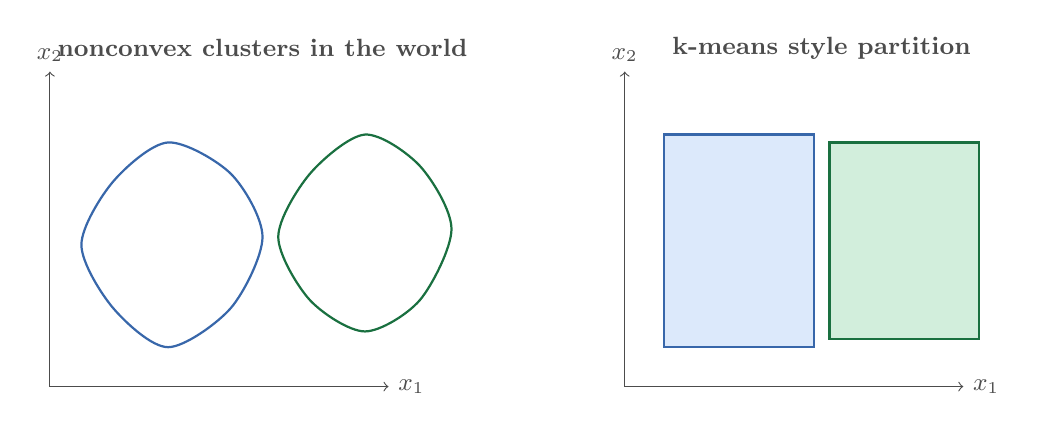
\begin{tikzpicture}[font=\small]
%% Panel A: true nonconvex clusters
\begin{scope}
  \draw[->,black!70] (0,0) -- (4.3,0) node[right] {$x_1$};
  \draw[->,black!70] (0,0) -- (0,4.0) node[above] {$x_2$};
  \draw[c4kmfTrue1,thick]
    plot[smooth cycle] coordinates {(0.8,1.0)(1.5,0.5)(2.3,1.0)(2.7,1.9)(2.3,2.7)(1.5,3.1)(0.8,2.6)(0.4,1.8)};
  \draw[c4kmfTrue2,thick]
    plot[smooth cycle] coordinates {(3.3,1.1)(4.0,0.7)(4.7,1.1)(5.1,2.0)(4.7,2.8)(4.0,3.2)(3.3,2.7)(2.9,1.9)};
  \node[black!70,font=\small\bfseries] at (2.7,4.3) {nonconvex clusters in the world};
\end{scope}
%% Panel B: k-means rectangular partition
\begin{scope}[xshift=7.3cm]
  \fill[c4kmfPart1] (0.5,0.5) rectangle (2.4,3.2);
  \fill[c4kmfPart2] (2.6,0.6) rectangle (4.5,3.1);
  \draw[->,black!70] (0,0) -- (4.3,0) node[right] {$x_1$};
  \draw[->,black!70] (0,0) -- (0,4.0) node[above] {$x_2$};
  \draw[c4kmfTrue1,thick] (0.5,0.5) rectangle (2.4,3.2);
  \draw[c4kmfTrue2,thick] (2.6,0.6) rectangle (4.5,3.1);
  \node[black!70,font=\small\bfseries] at (2.5,4.3) {k-means style partition};
\end{scope}
\end{tikzpicture}%
}
\caption{k-means is not a universal clustering truth machine. When cluster shape matters, the method's geometric bias can force a misleading partition.}
\label{fig:kmeans-failure}
\end{figure}

\section{Clustering Validity and the Danger of Naming Clusters Too Fast}

A clustering algorithm produces a partition. That partition is geometrically defined by the algorithm's notion of similarity, the number of clusters chosen, the initialization, and the features provided. None of those choices is neutral, and none guarantees that the resulting groups correspond to anything meaningful in the world.

Three levels of interpretation should be kept distinct. Each makes a stronger claim than the one before.

\textbf{Geometric grouping.} A clustering is valid in a narrow sense if the groups are internally coherent under the chosen metric. This is testable: intra-cluster distances should be small relative to inter-cluster distances under that metric. Silhouette scores and related diagnostics measure exactly this. But geometric validity says nothing about whether the groups mean anything.

\textbf{Operational usefulness.} A clustering is operationally useful if acting on it produces better outcomes than ignoring it. A segmentation of students into three groups is useful if the three groups genuinely benefit from different kinds of support, regardless of whether they correspond to any natural social or psychological category. Usefulness is measured by downstream outcomes, not by the algorithm's internal objective.

\textbf{Causal or social interpretation.} Naming a cluster is a stronger act than finding it. A label like ``students who lack intrinsic motivation'' or ``customers who are price-insensitive'' asserts a causal story or a social category. That label cannot be read off the clustering. It requires external validation: interviews, longitudinal follow-up, or theory that connects the geometric group to the label.

\begin{failurebox}
A common pattern: researchers run k-means on a student dataset, find three clusters, label them ``engaged,'' ``struggling,'' and ``disengaged,'' and then report policy recommendations as if those labels were real categories. The algorithm found a geometric partition; the labels are a narrative imposed afterward. If the partition is sensitive to initialization or feature scaling, the narrative is doubly fragile.
\end{failurebox}

\begin{example}[Clustering of Customer Data]
An e-commerce team clusters purchasing histories into five groups and labels them ``deal hunters,'' ``brand loyalists,'' and ``impulse buyers.'' The labels feel intuitive. But stability analysis reveals that three of the five clusters change substantially when the clustering is rerun with a different random seed. The geometric groups were artifacts of initialization, not stable population structure. The labels were named before the groups were tested.
\end{example}

The right habit is to treat any cluster as provisional until three questions are answered. Is the partition stable under small perturbations of the data and initialization? Does it support the operational decisions it will be used to justify? And what external evidence would be needed before a causal or social interpretation could be defended?

\begin{thinkingtool}
\textbf{Cluster naming discipline.} Describe clusters by their measurable properties first---average feature values, distinguishing coordinates, sample size. Name them with social or causal labels only after external validation. A cluster labeled ``high-risk'' that is defined only geometrically is not a validated risk group; it is a starting hypothesis.
\end{thinkingtool}

\section{Dimensionality Reduction as a Lens}

Another unsupervised goal is dimensionality reduction. Rather than grouping examples, we represent them with fewer coordinates while preserving important structure. Principal component analysis (PCA) is the standard example. It finds directions in feature space along which the data varies most and projects the data onto those directions.

PCA is best taught here not as a competitor to predictive methods but as a lens: a geometric summary, a useful preprocessing or inspection tool, and a reminder that simplified views are still model choices.

PCA is scale-sensitive. A feature measured in much larger numerical units can dominate the first principal component. Standardize features first when the units are not already comparable. On the shared student-profile cloud, the first component mainly tracks raw clicks unless the features are standardized; after standardization, it can reflect the click-versus-lateness tradeoff.

\begin{mathlens}
For centered data \(x_1,\ldots,x_n\), a one-dimensional PCA direction \(u\) with \(\|u\|_2=1\) can be found by maximizing the projected variance
\[
\frac{1}{n}\sum_{i=1}^n (x_i^\top u)^2.
\]
Equivalently, it minimizes the average squared reconstruction error after projection,
\[
\frac{1}{n}\sum_{i=1}^n \left\|x_i-(x_i^\top u)u\right\|_2^2,
\]
because pointwise
\[
\left\|x_i-(x_i^\top u)u\right\|_2^2=\|x_i\|_2^2-(x_i^\top u)^2,
\]
so the two expressions differ only by the additive constant \(\tfrac{1}{n}\sum_i \|x_i\|_2^2\), which does not depend on \(u\). Maximizing the first is therefore equivalent to minimizing the second, and PCA is choosing the direction that keeps the largest amount of variation after compression.
\end{mathlens}

\begin{figure}[t]
\centering
\definecolor{c4pcaBlue}{RGB}{56,103,170}
\definecolor{c4pcaAmber}{RGB}{184,92,16}
\resizebox{\linewidth}{!}{%
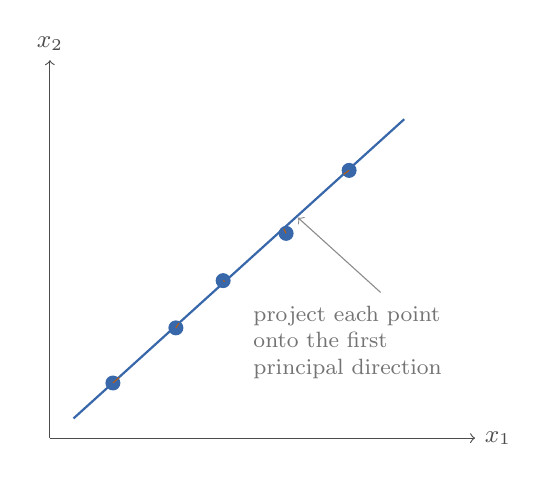
\begin{tikzpicture}[x=1cm, y=1cm, font=\small]
  \draw[->,black!70] (0,0) -- (5.4,0) node[right] {$x_1$};
  \draw[->,black!70] (0,0) -- (0,4.8) node[above] {$x_2$};
  %% Principal direction line (drawn before points so points render on top)
  \draw[c4pcaBlue,thick] (0.3,0.25) -- (4.5,4.05);
  %% Data points along the diagonal
  \foreach \px/\py in {0.8/0.7, 1.6/1.4, 2.2/2.0, 3.0/2.6, 3.8/3.4}
    \filldraw[fill=c4pcaBlue, draw=c4pcaBlue] (\px,\py) circle (2.5pt);
  %% Projection dashed lines (tiny perpendicular drops onto the line)
  \foreach \px/\py/\qx/\qy in {
    0.8/0.7/0.88/0.77,
    1.6/1.4/1.64/1.46,
    2.2/2.0/2.22/1.99,
    3.0/2.6/2.97/2.66,
    3.8/3.4/3.73/3.35}
  {
    \draw[c4pcaAmber, dashed, thin] (\px,\py) -- (\qx,\qy);
  }
  %% Annotation in the lower-right corner, well clear of the data diagonal
  \node[align=left, font=\footnotesize, black!55, anchor=north east] at (5.1,1.8)
    {project each point\\onto the first\\principal direction};
  %% Arrow pointing up-left from annotation toward the middle of the line
  \draw[->,thin,black!45] (4.2,1.85) -- (3.15,2.80);
\end{tikzpicture}%
}
\caption{PCA chooses a direction of large variation and projects the data onto it. It is a geometric summary, not ``compression magic.''}
\label{fig:pca-projection}
\end{figure}

For a small numeric intuition, imagine two centered features that mostly vary together. If increasing one feature almost always means increasing the other, most of the variation lies along a diagonal direction. PCA captures that shared direction first. A two-coordinate description can then be reduced to one dominant coordinate plus a smaller residual coordinate.

\begin{example}[Projecting One Point onto a Principal Direction]
Suppose the first principal direction is
\[
u=\frac{1}{\sqrt{2}}\begin{bmatrix}1\\1\end{bmatrix},
\]
and one centered data point is
\[
x=\begin{bmatrix}3\\1\end{bmatrix}.
\]
The one-dimensional PCA coordinate is the dot product
\[
x^\top u = \frac{3+1}{\sqrt{2}} = 2\sqrt{2}.
\]
Projecting back onto the principal direction gives
\[
(x^\top u)u = 2\sqrt{2}\cdot\frac{1}{\sqrt{2}}\begin{bmatrix}1\\1\end{bmatrix}
= \begin{bmatrix}2\\2\end{bmatrix}.
\]
PCA keeps the dominant diagonal component of the point and discards the residual orthogonal variation. That is the precise sense in which PCA compresses: it preserves some directions and throws away others.
\end{example}

\begin{advancednote}
The unsupervised landscape is broader than k-means and PCA. DBSCAN and hierarchical clustering are often better when cluster shape or nested structure matters; t-SNE and UMAP are mainly visualization tools. They can be highly informative, but they should not be treated as truth machines.
\end{advancednote}

\begin{table}[t]
\centering
\small
\setlength{\tabcolsep}{4pt}
\begin{tabular}{L{2.63cm}L{2.79cm}L{4.54cm}}
\toprule
Method family & Best when & Main warning \\
\midrule
Single tree & You need explicit branching logic and readable rules & A single tree can be unstable and overly sensitive to the sample \\
Random forest & Tabular data is strong and you want a safer default than one tree & Interpretation becomes weaker because the vote is spread across many trees \\
Boosted trees & You want strong accuracy on structured data and can tune carefully & More tuning-sensitive; easy to overfit if pushed too far \\
SVM & A wide-margin linear boundary is plausible in the current feature space & It depends on the representation; it will not repair missing structure by itself \\
Naive Bayes & Many sparse features, limited data, or a transparent class-conditional baseline & Independence assumptions and calibration must be checked \\
k-NN & Similar cases should borrow labels through a defended distance rule & Scaling and feature geometry are the model itself \\
Clustering/PCA & You have no labels and want organization, grouping, or compression & The result is a summary, not a discovered truth \\
\bottomrule
\end{tabular}
\caption{A compact synthesis helps students choose the next family without treating method names as interchangeable.}
\label{tab:chapter4-family-synthesis}
\end{table}

\section{Chapter Artifact: A Structure Diagnosis Sheet}

By the end of this chapter, the reader should be able to explain not only which method to try next but why that method matches the failure pattern of the linear baseline. Chapter~\ref{ch:linear-models} named the first serious model to try. This chapter names the reason to leave it. The chapter should end with one diagnosis, not a shopping list of unrelated methods.

\begin{table}[t]
\centering
\small
\setlength{\tabcolsep}{4pt}
\begin{tabular}{L{3.25cm}L{6.98cm}}
\toprule
Diagnosis field & What must be written clearly \\
\midrule
Seven-question focus & Questions 4, 5, and 6: identify the missing structure, choose the next justified baseline family, and state what evidence would support the move \\
Baseline failure & What the linear model is getting wrong and on what kind of examples \\
Structural hypothesis & Conditional logic, margin structure, class-conditional probabilistic structure, local similarity, or unlabeled organization \\
Candidate family & Tree, ensemble, SVM, Naive Bayes, nearest-neighbor, clustering, or dimensionality reduction method \\
Representation dependency & Which feature choices or scaling rules matter most for this family \\
Main risk & Instability, weak geometry, cluster overinterpretation, or another failure mode \\
Evidence needed & What validation or inspection result would justify moving beyond the baseline \\
Interpretation boundary & What the method's output does and does not justify claiming \\
\bottomrule
\end{tabular}
\caption{The chapter should end with a structural diagnosis, not with method shopping.}
\label{tab:structure-diagnosis-sheet}
\end{table}

\begin{example}[Filled Structure Diagnosis Sheet]
\textbf{Seven-question focus.} Questions 4 (representation/structure), 5 (next baseline), 6 (evidence).

\textbf{Baseline failure.} The logistic-regression baseline on student-support messages reaches recall 0.74 at the budgeted top-15\% threshold but loses ground on two slices: (a) messages that combine ``personal hardship'' phrases with ``deadline'' phrases (recall 0.46), and (b) short messages with strong sender history but weak lexical content (recall 0.61). The model is missing the way features \emph{combine} for some students.

\textbf{Structural hypothesis.} The decision is conditional, not linear. ``Personal hardship'' raises urgency only when paired with deadline pressure; sender history matters only when message content is sparse. A weighted-sum scorer cannot represent the AND-style interaction without explicit interaction features.

\textbf{Candidate family.} A shallow gradient-boosted tree ensemble. Trees represent conditional logic natively; boosting reduces variance from individual splits while keeping the structural pattern interpretable.

\textbf{Representation dependency.} Categorical features (sender tier, message channel) should remain as categories rather than one-hot expansions; tree splits handle them directly. Numeric features need no scaling.

\textbf{Main risk.} Tree ensembles can latch onto spurious interactions when slices are small. The hardship-plus-deadline slice has only 240 examples, so the tree may discover a brittle rule that does not generalize.

\textbf{Evidence needed.} A held-out evaluation that shows boosted trees beat logistic regression \emph{on the two failing slices} (not just on the overall metric), under the same evaluation plan from Chapter~\ref{ch:evaluation-discipline}, with the slice-level paired confidence interval clearly above zero.

\textbf{Interpretation boundary.} A tree's discovered split (``hardship $\wedge$ deadline'') describes a regularity in the available data; it does not justify a causal claim about which combination triggers urgency. The next step if the tree wins is a small targeted human review of flagged messages to verify the rule is meaningful, not coincidental.
\end{example}

\begin{thinkingtool}
\textbf{Structure diagnosis sheet.} Before changing model families, write down what the baseline missed, what structural hypothesis now seems plausible, why a tree, neighbor, or unsupervised method matches that hypothesis, and what evidence would justify the move.
\end{thinkingtool}

\section{Common Mistakes with Structural Methods}

The recurring mistakes here are conceptual rather than computational. Readers treat trees as automatically interpretable even when depth or boosting has made them opaque. They read feature importance as causation. They ignore scale in distance-based models even though geometry depends on units. They believe clusters too quickly. They treat a low-dimensional plot as the data's true structure. And they skip the baseline logic that should explain what the new family actually captures.

\section{Looking Ahead}

This chapter broadened structure beyond one weighted sum to branches, margins, probabilistic baselines, neighborhoods, and low-dimensional views. The next chapter makes the data itself explicit: how examples, labels, class balance, annotation quality, and acquisition strategy shape what any later model can learn.

\section*{Chapter Summary}

This chapter treated model choice as structural diagnosis. When a linear baseline fails, the important question is not whether more complexity is needed but what form the missing structure takes. Trees and ensembles address region-specific decision logic. SVMs address robust geometric separation. Naive Bayes introduces the generative perspective---modeling class-conditional feature distributions rather than decision boundaries---and provides a fast, interpretable probabilistic baseline. Nearest-neighbor methods treat similarity itself as the model. Clustering and dimensionality reduction address organization when labels are absent. The recurring lesson is that representation still matters: geometry, scaling, impurity, and cluster shape are part of the model, not preprocessing details.

\begin{studyquestions}
\item Why is ``what kind of structure is missing?'' a better opening question than ``which classical method comes next?'' 
\item Why should trees be understood as models for conditional logic rather than merely as nonlinear models?
\item Why is the notion of distance the real modeling choice in nearest-neighbor methods?
\item Why does maximizing margin make an SVM more robust than a separator that merely classifies correctly?
\item Why does Naive Bayes classify well despite violating the conditional independence assumption?
\item When is Naive Bayes a better structural choice than a tree or SVM?
\item Why should clusters be interpreted more cautiously than labeled classes?
\item What would count as evidence that a tree, neighbor, or unsupervised method is justified beyond the linear baseline?
\end{studyquestions}

\begin{exercises}
\item \exercisetag{Concept}{Core}Give a real-world example of a problem that naturally sounds like a branching rule rather than a single weighted score. Explain why.
\item \exercisetag{Calculation}{Core}Using Table~\ref{tab:tree-split-data}, verify the impurity reduction for the two candidate root splits by hand.
\item \exercisetag{Diagnosis}{Core}Explain why classification trees and regression trees share the same recursive structure even though their leaf predictions are different.
\item \exercisetag{Concept}{Core}Classify the query student described just before Table~\ref{tab:knn-scaling-data} with $k=1$ and $k=3$ before and after scaling. Explain why the prediction changes.
\item \exercisetag{Concept}{Intermediate}For the one-dimensional SVM example in this chapter, explain why the threshold at \(x=2\) has a larger margin than a threshold at \(x=1.5\).
\item \exercisetag{Concept}{Intermediate}Using the binary-case identity $G=2p(1-p)$, compute the Gini impurity of nodes with positive-class fractions $0.1$, $0.5$, and $0.9$. Explain which node is hardest to split cleanly.
\item \exercisetag{Calculation}{Intermediate}Run one k-means iteration by hand for the points $(1,1)$, $(1,2)$, $(4,4)$, and $(5,4)$ with initial centers $c_1=(1,1)$ and $c_2=(5,4)$. State the assignments and the recomputed centers.
\item \exercisetag{Design}{Intermediate}Sketch a small 2D dataset for which a shallow tree should beat a linear model for the right reason. State clearly what threshold or interaction the tree captures.
\item \exercisetag{Concept}{Intermediate}Why might a random forest outperform a single decision tree even though both are built from the same basic building block?
\item \exercisetag{Concept}{Intermediate}Give one example in which clustering could be useful for exploration and one example in which clustering could be dangerously overinterpreted.
\item \exercisetag{Design}{Intermediate}Write language-neutral pseudocode for 1-nearest-neighbor classification using Euclidean distance, then explain how the returned label can change after rescaling one feature.
\item \exercisetag{Design}{Intermediate}Use Table~\ref{tab:structure-diagnosis-sheet} to write a one-page diagnosis for a failed linear baseline in either student support, spam filtering, or another application of your choice. If you are carrying one case through the book, extend the baseline design sheet from the previous chapter instead of inventing a fresh failure.
\item \exercisetag{Implementation}{Core}Implement 1-nearest-neighbor classification from scratch on the dataset in Table~\ref{tab:knn-scaling-data} (or a fresh 2D dataset of about 20 points and 2 classes). Write \verb|knn_predict(X_train, y_train, X_query)| using only \verb|numpy| broadcasting for the Euclidean distances. Predict labels for a $50 \times 50$ grid covering the data range, twice: once on raw features and once after standardizing each column to zero mean and unit variance. Plot the two decision regions side by side and identify at least one query point whose predicted label flips after scaling.
\item \exercisetag{Implementation}{Intermediate}Build a depth-2 classification tree by hand-coded loops on a 2D dataset of your choice (e.g., the XOR-like construction in your sketch from the earlier exercise). The tree should at each node enumerate every candidate (feature, threshold) split, score it by Gini impurity, and pick the best. Report the chosen splits, plot the decision regions, and verify that the tree achieves zero training error on a constructed XOR-style example where any single linear separator fails.
\end{exercises}

\begin{challengeexercises}
\item \exercisetag{Design}{Advanced}Construct a tiny binary classification dataset in two dimensions for which a linear separator performs poorly but a depth-2 decision tree performs perfectly. Explain the split sequence.
\item \exercisetag{Concept}{Advanced}Suppose a 1-nearest-neighbor classifier gives unstable predictions when one feature is added to the dataset. Give two different explanations for why this could happen.
\item \exercisetag{Concept}{Advanced}A team clusters user behavior data into four groups and labels them ``leaders,'' ``followers,'' ``at risk,'' and ``disengaged.'' Explain why this move from mathematical grouping to substantive naming requires additional evidence, and describe what evidence would help.
\item \exercisetag{Diagnosis}{Advanced}Give a clustering result that looks convincing on one 2D plot but should still fail a stability sanity check. Explain what change in scaling, initialization, or sampling would reveal the weakness.
\item \exercisetag{Concept}{Advanced}DBSCAN, hierarchical clustering, t-SNE, and UMAP sit alongside k-means and PCA for different reasons. Give one sentence each on what problem characteristic might make you look beyond k-means.
\end{challengeexercises}
